\documentclass{gtpart}
\usepackage{amsmath,amssymb,amsthm,stmaryrd}
\usepackage[all]{xy}
\usepackage{tikz}
\usepackage{url}
%\usepackage{setspace}
%\doublespacing

\title{The power operation structure on the $K(1)$-localization of $E_2$}
\author{Yifei Zhu}
\givenname{Yifei}
\surname{Zhu}
%\address{Department of Mathematics\\University of Minnesota\\Minneapolis, MN 55455\\USA}
%\email{zyf@umn.edu}

%\subject{primary}{msc2000}{55P99}
%\subject{secondary}{msc2000}{55Q99}

\bibliographystyle{gtart}
\parskip 0.7pc
\parindent 0pt

\newtheorem{thm}{Theorem}
\newtheorem{cor}[thm]{Corollary}
\newtheorem{prop}[thm]{Proposition}
\newtheorem{lem}[thm]{Lemma}
\theoremstyle{definition}
\newtheorem{defn}[thm]{Definition}
\theoremstyle{remark}
\newtheorem{rmk}[thm]{Remark}
\newtheorem{exam}[thm]{Example}
\newtheorem{case}[thm]{Case}
\newtheorem{slogan}[thm]{Slogan}
\newtheorem{ques}[thm]{Question}

\def\co{\colon\thinspace}
\newcommand{\mb}[1]{\mathbb{#1}}
\newcommand{\mf}[1]{\mathfrak{#1}}

\newcommand{\NB}[1]{{\bf (NB: #1)}}

\newcommand{\Ext}{\ensuremath{{\rm Ext}}}
\newcommand{\Coext}{\ensuremath{{\rm Coext}}}
\newcommand{\Hom}{\ensuremath{{\rm Hom}}}
\newcommand{\Tor}{\ensuremath{{\rm Tor}}}
\newcommand{\Ind}{\ensuremath{{\rm Ind}}}
\newcommand{\Res}{\ensuremath{{\rm Res}}}
\newcommand{\colim}{\ensuremath{\mathop{\rm colim}}}
\newcommand{\hocolim}{\ensuremath{\mathop{\rm hocolim}}}
\newcommand{\holim}{\ensuremath{\mathop{\rm holim}}}
\newcommand{\overto}{\mathop\rightarrow}
\newcommand{\overfrom}{\mathop\leftarrow}
\newcommand{\into}{\mathop\hookrightarrow}
\newcommand{\onto}{\mathop\twoheadrightarrow}
\newcommand{\longoverto}{\mathop{\longrightarrow}}
\newcommand{\Irr}{\ensuremath{\mathop{\rm Irr}}}
\newcommand{\Rep}{\ensuremath{\mathop{\rm Rep}}}
\newcommand{\Map}{\ensuremath{{\rm Map}}}
\newcommand{\GL}{{\rm GL}}
\newcommand{\Uni}{{\rm U}}
\newcommand{\BU}{{\rm BU}}
\newcommand{\Sp}{{\cal S}p}
\newcommand{\Sym}{{\rm Sym}}
\newcommand{\thh}{{\rm thh}}
\newcommand{\TAF}{{\rm TAF}}
\newcommand{\TAQ}{{\rm TAQ}}
\newcommand{\End}{{\rm End}}
\newcommand{\Aut}{{\rm Aut}}
\newcommand{\md}{{\rm mod}}
\newcommand{\As}{{\cal A}s}
\newcommand{\LT}{{\rm LT}}
\newcommand{\Spec}{{\rm Spec}}
\newcommand{\Spf}{{\rm Spf}}
\newcommand{\tmf}{{\rm tmf}}
\newcommand{\eo}{{\rm eo}}
\newcommand{\TMF}{{\rm TMF}}
\newcommand{\Ell}{{\cal E}ll}
\newcommand{\Lie}{{\rm Lie}}
\newcommand{\Sh}{{\rm Sh}}
\newcommand{\HF}{{\rm H}{\mb F}}
\newcommand{\cF}{\overline {\mb F}}
\newcommand{\cQ}{\overline {\mb Q}}

\newcommand{\eilm}[1]{\ensuremath{{\mb H} #1}}
\newcommand{\smsh}[1]{\ensuremath{\mathop{\wedge}_{#1}}}
\newcommand{\tens}[1]{\ensuremath{\mathop{\otimes}_{#1}}}
\newcommand{\susp}{\ensuremath{\Sigma}}
\newcommand{\mapset}[3]{\ensuremath{\left[#2,#3\right]_{#1}}}
\newcommand{\form}[2]{\ensuremath{\left\langle#1,#2\right\rangle}}
\newcommand{\bilin}[2]{\ensuremath{\left(#1,#2\right)}}
\newcommand{\comp}[1]{\ensuremath{#1^\wedge}}
\newcommand{\loca}[3]{\ensuremath{L^{#1}_{#2}(#3)}}
\newcommand{\tc}[3]{\ensuremath{\Omega_{#2 / #1}^{#3}}}
\newcommand{\atc}[3]{\ensuremath{\L_{#2 / #1}^{#3}}}

\newcommand{\xym}[1]{
\vskip 0.7pc
\centerline{\xymatrix{#1}}
\vskip 0.7pc
}

\newcommand{\DL}{{\rm DL}}
\newcommand{\CA}{{\cal A}}
\newcommand{\Mod}{{\rm Mod}}
\newcommand{\Alg}{{\rm Alg}}
\newcommand{\Frob}{{\rm Frob}}
\newcommand{\CO}{{\cal O}}
\newcommand{\DF}{{{\rm DefFrob}_\Gamma}}
\newcommand{\Model}{{\rm Model}}
\newcommand{\Gm}{{{\mb G}_m}}
\newcommand*{\longhookrightarrow}{\ensuremath{\lhook\joinrel\relbar\joinrel\rightarrow}}

\begin{document}

\begin{abstract}
  We give an overview of the structure of the Dyer-Lashof theories 
  associated to Morava $E$-theories, and to their $K(1)$-localizations 
  in particular, leading to the connection with explicit calculations of 
  elliptic curves when the $E$-theory is an elliptic cohomology theory.
\end{abstract}

\maketitle
\section{Introduction}
\label{sec:intro}


The study of cohomology operations has become central to algebraic 
topology since the 1950s, with applications to problems such as vector 
fields on spheres, and the non-existence of elements of Hopf invariant 
one, the latter of which has impact on the author most recently felt 
when he tried to answer a question raised by students in a calculus 
class (interested readers might see \cite{massey}).  


\subsection{Dyer-Lashof theories}
\label{subsec:DL}

One organizing principle for understanding the structure among 
operations is through the {\em algebraic theories} of operations.  An 
{\em (algebraic) theory} is a category $T$ with object set 
$\{T^0,T^1,T^2,...\}$, together with {\em projection maps} 
$\pi_i\co T^n \to T^1$ for all $n \geq 1$, $1 \leq i \leq n$ such that 
$T(T^k,T^n) \xrightarrow{\pi_i} \prod_{i=1}^n T(T^k,T^1)$ is a 
bijection for all $k$ and $n$, ie $T^n$ is isomorphic to the $n$-fold product 
of $T^1$.  Also there is a canonical map $T^0 \to T^1$.  A {\em morphism 
of theories} is a functor $\phi\co T \to T'$ which preserves the product 
structure of a theory, ie $\phi(T^k) = T'^k$ and 
$\phi(T^k \stackrel{\pi_i}{\longrightarrow} T^1) = T'^k \stackrel{\pi_i'}{\longrightarrow} T'^1$.  

A {\em model} of the theory $T$ is a functor $A\co T \to \rm{Set}$ which 
preserves finite products.  It can be thought of as the 
underlying set $X = A(T^1)$ together with operations 
$\psi_f\co X^k \to X^n$ corresponding to each $f \in T(T^k,T^n)$.  
In particular, a {\em free model} on $n$ generators is the model 
$F_T(n)$ defined by $F_T(n)(T^m) = T(T^n,T^m)$.  We write $\Model_T$ 
for the category of models of $T$.  For example, let $R$ be 
a commutative ring, and let $F$ be the full subcategory of 
the category of commutative $R$-algebras having as objects $\{F_0,F_1,F_2,...\}$, where 
$F_0 = R$ and $F_n = R[x_1,...,x_n]$ for $n \geq 1$.  We then have 
the theory of commutative $R$-algebras $C_R = F^{\rm op}$.  

A {\em commutative operation theory} (COT) is a triple $(T,R,\phi)$ 
consisting of a theory $T$, a commutative ring $R$, and a morphism 
$\phi\co C_R \to T$ of theories, such that the induced functor $\phi^*\co 
\Model_T \to \Model_{C_R}$ commutes with finite coproducts.  
In other words, every $T$-model has an underlying structure of 
a commutative $R$-algebra, and coproducts in $\Model_T$ are computed 
by tensor products over $R$.  We will write $R\{x_1,...,x_n\}$ for 
a free $T$-model on $n$ generators, and we have $R\{x_1,...,x_n\} \cong 
R\{x_1\} \otimes_R \cdots \otimes_R R\{x_n\}$.  

We next introduce grading to a theory by having a fixed set 
$C$ of {\em colors}.  Let ${\mb N}[C]$ be the free commutative monoid 
on $C$.  A $C$-graded theory $T$ is then a category with object set 
$\{T^d\}_{d \in {\mb N}[C]}$, together with, for each 
$d = \sum_{c \in C} d_c[c] \in {\mb N}[C]$, a specified identification of 
$T^d$ with the product $\prod_{c \in C} (T^{[c]})^{d_c}$.  
In particular, we can define a graded COT as 
a triple $(T,R_*,\phi)$ similarly as above, with $T$ a $\mb Z$-graded theory 
and $R_*$ a graded commutative ring.  

For a graded COT $(T,R_*,\phi)$, let ${\cal A}(c,d)$ 
be the set of elements $f \in R_*\{x\}_d = T(T^{[c]},T^{[d]})$ which are 
primitive under the comultiplication $R_*\{x\} \xrightarrow{x \mapsto x_1 + x_2} R_*\{x_1,x_2\}$, where $|x| = |x_1| = |x_2| = c$.  
Such $f \in {\cal A}(c,d)$ give rise to additive functions $A_c \to A_d$ 
natural in the model $A$, and in particular the element $x \in R_*\{x\}_c$ 
corresponds to the identity map on $A_c$.  Thus we obtain a category $\cal A$ 
of additive operations, whose object set is $\mb Z$, the set of colors of 
our graded COT.  

For example, let $T = O_{H{\mb F}_p}$ be the graded COT given by 
\[
 T(O_{H{\mb F}_p}^{[c_1]+\cdots+[c_m]},O_{H{\mb F}_p}^{[d_1]+\cdots+[d_n]}) = [K({\mb F}_p,c_1) \times \cdots \times K({\mb F}_p,c_m), K({\mb F}_p,d_1) \times \cdots \times K({\mb F}_p,d_n)],
\]
where we use homotopy classes of maps, and use the convention that $K({\mb F}_p,c) = *$ for $c<0$.  
Then $\Model_{O_{H{\mb F}_p}}$ is the category of unstable algebras over the mod-$p$ Steenrod algebra, 
and ${\cal A}(c,d)$ is the set of additive operations $H^c(-;{\mb F}_p) \to H^d(-;{\mb F}_p)$, which, 
for $p=2$, are linear combinations of monomials as admissible composites of Steenrod operations having excess no more than $c$.  

Having the COT describing cohomology operations on spaces, we next 
consider one describing operations on spectra.  Given a 
commutative $S$-algebra $R$ ($S$ is the sphere spectrum), the {\em Dyer-Lashof theory} $\DL_R$ is 
the $\mb Z$-graded theory $T$ defined by 
\[
 T(T^{[c_1]+\cdots+[c_m]},T^{[d_1]+\cdots+[d_n]}) = h\Alg_R \Big({\mb P}_R \big(R \wedge (S^{d_1} \vee \cdots \vee S^{d_n}) \big), {\mb P}_R \big(R \wedge (S^{c_1} \vee \cdots \vee S^{c_m}) \big) \Big),
\]
where $\mb P$ is the free algebra functor defined by ${\mb P}(X) = 
\bigvee_{m \geq 0} {\mb P}^m(X) = \bigvee_{m \geq 0} X^{\wedge m}/\Sigma_m$.  
We have the identification ${\mb P}^m (S^c) \cong B\Sigma_m^{cV_m}$, 
where $V_m = {\mb R}^m$ equipped with the $\Sigma_m$-action given by 
permuting coordinates, and $c \in {\mb Z}$, so that the right-hand 
side is the Thom spectrum of a virtual bundle.  The free theories 
are given by 
\[
 F([c_1]+\cdots+[c_m])_{[d]} = \pi_d {\mb P}_R \big( R \wedge (S^{c_1} \vee \cdots \vee S^{c_m}) \big) = \pi_d \Big( R \wedge \big({\mb P}(S^{c_1}) \vee \cdots \vee {\mb P}(S^{c_m})\big) \Big).
\]
Moreover, if $\pi_*R\wedge{\mb P}(S^c)$ are flat as left $\pi_*R$-modules, $\DL_R$ becomes a COT.  
The significance of $\DL_R$ is that it describes all homotopy operations on commutative $R$-algebras: 
\[
 \DL_R([c],[d]) = h\Alg_R \big( {\mb P}_R(R \wedge S^d), {\mb P}_R(R \wedge S^c) \big) = \{\pi_c(-) \to \pi_d(-)\}.
\]
For example, if $R$ is a ring (no longer a spectrum) containing ${\mb F}_2$, there is a complete description of $\DL_{HR}$, which is a COT.  
A $\DL_{HR}$-model is a graded commutative $R$-algebra $A_*$, equipped with functions $Q^s\co A_c \to A_{c+s}$ for all 
$s, c \in {\mb Z}$, satisfying a bunch of properties, eg the Cartan formula and the Adem relations.  


\subsection{Dyer-Lashof theories associated to Morava $E$-theories}
\label{subsec:DL}

One organizing principle for understanding large-scale phenomena in 
homotopy theory is through the {\em chromatic filtration} (cf 
\cite{tafoverview,coctalos}), which corresponds to a stratification 
of the moduli stack of formal groups into layers according to height.  
The formal groups come about in terms of formal group laws which express the 
first Chern class of the tensor product of two line bundles in terms 
of the first Chern classes of the individual line bundles, given any 
complex oriented cohomology theories.  Morava $E$-theories are 
universal among cohomology theories at each fixed layer of this 
filtration.  More precisely, for each formal group law $F$ of height 
$n<\infty$ over a perfect field $k$ of characteristic $p$, there 
is an $E_\infty$ ring spectrum $E_n(k,F)$ whose homotopy groups are 
the Lubin-Tate ring ${\mb W}k \llbracket v_1,...,v_{n-1} \rrbracket$ 
which is universal among complete local rings with residue field $k$ 
carrying a formal group law whose reduction to $k$ is $F$.  

Given a Morava $E$-theory $E_*$, there is an associated Dyer-Lashof 
theory $\DL_{E_*}$ describing all $E$-cohomology operations, which is 
defined similarly as above, except that we need to apply a certain 
localization to have good values of $E_* B\Sigma_m$ (which is mostly torsion 
for a general ring spectrum $E$).  In particular the free model on 
one generator is $E_*\{x_c\} = \bigoplus_{m \geq 0} E_*^\wedge (B\Sigma_m^{cV_m})$, 
where the completed theory $E_*^\wedge (-)$ reflects the localization.  

In the following sections we discuss the structure of $\DL_{E_*}$.  As 
is explained right at the beginning of \cite{Andu}, we hope 
to learn about the conjectural geometry of the theories $E_n$ by 
examining cohomology operations -- in particular, power operations -- along the lines of ordinary rational homology or $K$-theory (which 
are the initial cases $E_0$ and $E_1$).  


\section{The structure of power operations}
\label{sec:at2ec}


Let $E_*$ be the Morava $E$-theory associated to a formal group 
$\Gamma$ of height $n < \infty$ over a perfect field $k$ of 
characteristic $p$.  Based on knowledge of the spectrum $E$, 
we study the structure of $\DL_{E_*}$, the $\mb Z$-graded Dyer-Lashof 
theory associated to $E_*$, which describes all homotopy operations 
on commutative $E$-algebras.  We restrict our attention to the 
degree 0 part $\DL_{E_0}$.  The main input comes from deformations 
of Frobenius, which we discuss below.  In particular, when 
$E$ is an elliptic spectrum, these are parametrized by finite 
subgroups of the formal group of the associated elliptic curve, 
and thus we may study the operations by doing calculations of 
elliptic curves.  


\subsection{Identifications of categories}
\label{subsec:id}

First we consider the additive operations.  Let $\CA$ be the set 
of additive elements in the free $\DL_{E_0}$-model on one generator 
$E_0\{x\} = \bigoplus_{m \geq 0} E_0^\wedge B\Sigma_m$.  Write 
$\CA_{[m]} \subset E_0^\wedge B\Sigma_m$ for the summand, and write 
$\CA_r = \CA_{[p^r]}$.  It turns out that $\CA_{[m]} = 0$ 
unless $m = p^r$ for some $r$ (cf \cite{strickland}).  Thus $\CA = \bigoplus_{r \geq 0} \CA_r$ 
is an associative (not necessarily commutative) graded ring 
with respect to a product given by ``composition of operations'', 
with the unit element given by the generator $x \in E_0\{x\}$ 
representing the identity operation.  Moreover, the category 
$\Mod_\CA$ of left $\CA$-modules naturally admits a tensor product.  

We formulate a category equivalent to $\Mod_\CA$, which is specific 
to Morava $E$-theories, using deformations of Frobenius.  Let $R$ be 
a complete local ring containing ${\mb F}_p$ with maximal ideal $\mf m$.  
If $A$ is an $R$-algebra, we write $\Frob^*\co \sigma^*A \to A$ for 
the map of $R$-algebras which fits into the diagram 
\begin{center}
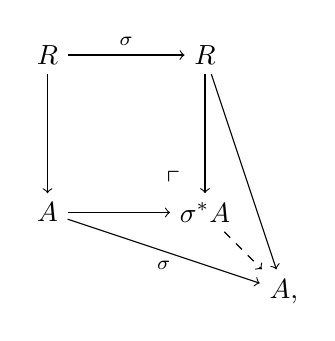
\begin{tikzpicture}
	\node (LT) at (0, 3) {$R$};
        \node (LB) at (0, 1) {$A$};
	\node (RT) at (2, 3) {$R$};
	\node (RB) at (2, 1) {$\sigma^*A$};
	\node (RB0) at (3, 0) {$A$,};
	\node at (1.6, 1.4) {$\ulcorner$};
	\draw [->] (LT) -- (LB);
	\draw [->] (LT) -- node [above] {$\scriptstyle \sigma$} (RT);
        \draw [->] (LB) -- (RB);
	\draw [->] (LB) -- node [below] {$\scriptstyle \sigma$} (RB0);
	\draw [->] (RT) -- (RB);
	\draw [->] (RT) -- (RB0);
	\draw [->, dashed] (RB) -- (RB0);
\end{tikzpicture}
\end{center}
where $\sigma$ sends an element to its $p$th power.  In particular, 
if $G$ is a formal group over $R$, there is an isogeny 
$\Frob\co G \to \sigma^*G$ of formal groups over $R$ defined by 
$\Frob^*\co \CO_{\sigma^*G} = \sigma^*\CO_G \to \CO_G$, 
$R \llbracket y \rrbracket \to R \llbracket x \rrbracket$ sending $y$ 
to $x^p$.  

A deformation of $\Gamma$ to $R$ is a triple $(G,i,\alpha)$ 
consisting of a formal group $G$ over $R$, an inclusion 
$i\co k \to R/\mf m$ and an isomorphism $\alpha\co G_0 \to i^*\Gamma$ 
of formal groups over $R/\mf m$.  And a $\star$-isomorphism 
$(G,i,\alpha) \to (G',i',\alpha')$ is an isomorphism 
$\phi\co G \to G'$ of formal groups over $R$ such that $i' = i$ and 
$\alpha' \circ \phi_0 = \alpha$.  We define $\DF(R)$ to be the category 
whose objects are deformations of $\Gamma$ to $R$, and whose morphisms 
are isogenies which are deformations of Frobenius, ie a morphism 
$(G,i,\alpha) \to (G',i',\alpha')$ is an isogeny $\phi\co G \to G'$ 
such that $i' = \sigma^r \circ i$ and 
$\alpha' \circ \phi_0 = \Frob^r \circ \alpha$ for some $r \geq 0$.  
In particular, $\phi$ is precisely a $\star$-isomorphism if $r = 0$.  

We then define a category $\Mod_\DF$ as follows, which is the category 
of sheaves of modules on $\DF = \{\DF(R)\}$.  An object $\cal F$ 
consists of 
\begin{enumerate}
\item for each complete local ring $R$ containing ${\mb F}_p$, a functor
\[
{\cal F}_R\co \DF(R)^{\rm op} \to \Mod_R,
\]
\item for each local homomorphism $f\co R \to R'$, a natural isomorphism 
\[
{\cal F}_f\co f^*{\cal F}_R \to {\cal F}_{R'}f^*,
\]
where the first $f^*$ is the functor $\Mod_R \to \Mod_{R'}$ of extending 
scalars along $f$, and the second 
$f^*\co \DF(R)^{\rm op} \to \DF(R')^{\rm op}$ is induced by $f$ (as 
$\DF(-)$ is a functor),
\end{enumerate}
such that they admit coherent natural isomorphisms
\begin{enumerate}
\item[(a)] ${\cal F}_{\rm id} \cong {\rm id}$ and 
${\cal F}_{gf} \cong {\cal F}_g(f^*) \circ g^*({\cal F}_f)$.  
\end{enumerate}
And a morphism $\eta\co {\cal F} \to {\cal G}$ is a collection of 
natural transformations $\eta_R\co {\cal F}_R \to {\cal G}_R$ such that 
${\cal G}_f \circ f^*(\eta_R) = \eta_{R'}(f^*) \circ {\cal F}_f$.  
Moreover, this is a tensor category with ${\cal F} \otimes {\cal G}$ 
given by $({\cal F} \otimes {\cal G})_R(G) = 
{\cal F}_R(G) \otimes_R {\cal G}_R(G)$.  

\begin{thm}[\cite{lpo}]
There is an equivalence of tensor categories $U\co \Mod_\CA \to \Mod_\DF$.
\end{thm}

Next we consider $\Model_{\DL_{E_0}}$, the category of models for the 
theory $\DL_{E_0}$, on which $\CA$ acts so that 
there is a forgetful functor $\Model_{\DL_{E_0}} \to \Mod_\CA$ along 
which the coproduct of $\DL_{E_0}$-models and the tensor product of 
$\Mod_\CA$ agree.  We define a category $\Alg_\DF$ as follows.  
An object $\cal B$ is a ring object in $\Mod_\DF$ which satisfies
\begin{enumerate}
 \item[(b)] the {\em Frobenius congruence}, ie the diagram
\begin{center}
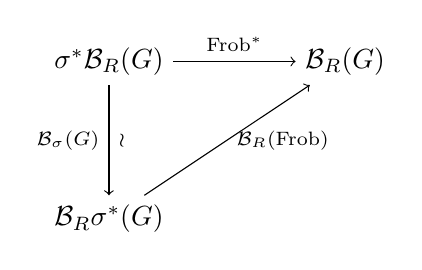
\begin{tikzpicture}
	\node (LT) at (0, 2) {$\sigma^*{\cal B}_R(G)$};
        \node (LB) at (0, 0) {${\cal B}_R\sigma^*(G)$};
	\node (RT) at (3, 2) {${\cal B}_R(G)$};
	\draw [->] (LT) -- node [left] {$\scriptstyle {\cal B}_\sigma(G)$} 
                           node [right] {$\scriptstyle \wr$} (LB);
	\draw [->] (LT) -- node [above] {$\scriptstyle \Frob^*$} (RT);
	\draw [->] (LB) -- node [right] {$\scriptstyle {\cal B}_R(\Frob)$} (RT);
\end{tikzpicture}
\end{center}
commutes for all complete local rings $R$ containing ${\mb F}_p$ and 
deformations $G$ of $\Gamma$ to $R$.  
\end{enumerate}
And morphisms are maps of ring 
objects.  An object ${\cal B}$ is said to be torsion free if 
${\cal B}_R(G)$ is $p$-torsion free for every $p$-torsion free $R$ 
and every deformation $G$ to $R$.  

\begin{thm}[\cite{lpo}]
There is a functor $U\co \Model_{\DL_{E_0}} \to \Alg_\DF$, and it 
restricts to an equivalence $U\co \Model_{\DL_{E_0}}^{\rm tf} \to 
\Alg_\DF^{\rm tf}$ of full subcategories of torsion free objects.
\end{thm}


\subsection{Deformations of Frobenius are parametrized by subgroups}
\label{subsec:subgp}

Having identified the categories, we now analyze the essential data 
encoded in $\Mod_\DF$ and $\Alg_\DF$, by studying the structure of 
the category $\DF(R)$ of deformations of Frobenius.  This turns out 
to be parametrized by subgroups of the deformations of $\Gamma$ to $R$.

Choosing a coordinate of a formal group $G$ over $R$, 
a degree (or rank) $d$ subgroup $K$ of $G$ is an effective divisor with 
$\CO_K = R \llbracket x \rrbracket / \big(f(x)\big)$ for some degree $d$ 
monic polynomial $f(x)$ such that $f(x_1 +_G x_2) \in \big(f(x_1),f(x_2)\big)$ 
and $f(x) \in (x)$, ie the group law of $G$ restricts to $K$ and 
$K$ contains the identity.  One can show that the homomorphism 
$[d]_G\co G \to G$ restricts to zero on $K$ (cf \cite{tateoort}).  
More concretely, this means that $f(x)$ must divide $[d]_G(x)$.  
As a consequence, subgroups of a formal group over a $p$-local 
ring must have degree $p^r$.  In particular, if $G$ is a formal 
group over a field $k$ of characteristic $p$, there is exactly 
one subgroup of degree $p^r$, given by $f(x) = x^{p^r}$, which 
is the kernel of $\Frob^r$.  

We have seen that in $\DF(R)$ the ``degree 1'' morphisms (when $r = 0$) 
are precisely the $\star$-isomorphisms of deformations.  
In general, including the cases when $r \geq 0$, $\DF(R)$ can 
be shown to be equivalent to the following category (cf \cite{lpo}).  
The objects are $\star$-isomorphism classes of deformations $[G]$.  
And the morphisms are $\star$-isomorphism classes of pairs $[G > K]$: 
the source of $[G > K]$ is $[G]$, and the target of $[G > K]$ 
is $[G/K]$, where $G/K$ is a deformation of $\Gamma$ with 
$i_{G/K} = \sigma^r \circ i_G$ ($p^r$ being the degree of $K$).  
Moreover, if $G/K \cong G'$, then $[G' > K'] \circ [G > K] = 
[G > K'']$, where $K''$ is the kernel of the composite 
$G \to G/K \cong G' \to G'/K'$.  Thus deformations of Frobenius 
with source $(G,i,\alpha)$ correspond {\em exactly} to finite 
subgroups of $G$.  

\begin{exam}
\label{ex:K}
Let $\Gamma$ be the multiplicative formal group over ${\mb F}_p$ 
of height 1.  For the multiplicative formal group $\Gm$ over a 
$p$-local ring $R$, since the formal group law is defined by 
$1 + (x_1 +_\Gm x_2) = (1 + x_1)(1 + x_2)$, inductively we have 
$[p^r](x) = (1 + x)^{p^r} - 1 = x^{p^r}$.  Thus the only subgroups 
of $\Gm$ are $\Gm [p^r]$ with $\CO_{\Gm [p^r]} = \CO_\Gm / (x^{p^r})$.  
Moreover, by the Lubin-Tate theorem (cf \cite{lubintate}), every object of $\DF(R)$ is 
$\star$-isomorphic to $\Gm$.  In particular, the set of 
$\star$-isomorphism classes of deformations of $\Gamma$ to $R$ 
is classified by the ring $\CO_{\rm univ} = {\mb Z}_p$, and we 
can take the universal deformation $G_{\rm univ}$ to be the 
multiplicative formal group over ${\mb Z}_p$.  Thus by functoriality, 
to describe an object ${\cal B} \in \Alg_\DF$, it is enough to give
\begin{enumerate}
\item a ${\mb Z}_p$-algebra $B = {\cal B}_{{\mb Z}_p}(\Gm)$, 
\item maps of ${\mb Z}_p$-algebras $\psi^{p^r}\co B \to B$ 
(corresponding to the isogenies $[p^r]\co \Gm \to \Gm$) such that 
\begin{enumerate}
 \item $\psi^1 = {\rm id}_B$ and $\psi^{p^r} \circ \psi^{p^s} = 
\psi^{p^{r+s}}$,
 \item $\psi^p(b) \equiv b^p$ mod $pB$.
\end{enumerate}
\end{enumerate}
(For comparison, the items are labelled as in the definitions of $\Mod_\DF$ and 
$\Alg_\DF$ above.)  We note as in \cite{cong} that this is a 
``$p$-typicalization'' of the original theorem of Wilkerson 
(cf \cite{wilkerson}), which characterizes the torsion free $\lambda$-rings 
in terms of congruences on the Adams operations at all primes.

More concretely, let $K$ be the complex $K$-theory spectrum.  Then 
for $B = \pi_0 A$, where $A$ is a $p$-complete $K$-algebra 
(commutative $K$-algebra such that $A \cong A_p^\wedge$), $\psi^p$ 
recovers the classical $p$th Adams operation.  On the other hand, 
if $B$ contains ${\mb F}_p$, then $\psi^p(b) = b^p$ is the 
classical Frobenius map on the ring of Witt vectors 
${\mb W} B = \Hom_{\Alg_{{\mb Z}_p}} (\Lambda,B)$, where 
$\Lambda = {\mb Z}_p [x_k, k \geq 0]$.  For more discussions on 
Lubin's theory of isogenies and the $p$-series of the multiplicative 
formal group, which underlies this example, see \cite[example 2.7]{Andu}.
\end{exam}

In general, the functor $X_r$, which associates to a ring $R$ the 
set of $\star$-isomorphism classes of pairs $[G > K]$ with $K$ a 
degree $p^r$ subgroup of $G$, is represented by the complete 
local ring $\CO_{X_r} = E^0 B\Sigma_{p^r}/I$, where 
$I = \sum_{0<i<p^r} {\rm Image}\big(E^0 B(\Sigma_i\times\Sigma_{p^r-i}) 
\xrightarrow{\text{transfer}} E^0 B\Sigma_{p^r}\big)$ is 
the {\em transfer ideal} (roughly speaking, the corresponding 
power operation should be additive, so modulo the ``extra terms'' 
in the Cartan formula).  This can be viewed as a 
generalization of the Lubin-Tate theorem for $\CO_{\rm univ} = 
\CO_{X_0}$.  Moreover, there are two ring homomorphisms $s^*$, 
$t^*\co \CO_{\rm univ} \to \CO_{X_r}$, where $s^*$ represents the 
source map $[G > K] \mapsto [G]$, and $t^*$ represents the target 
map $[G > K] \mapsto [G/K]$.  (In the example of multiplicative 
formal group, $\CO_{X_r} \cong \CO_{\rm univ}$ for all $r$, and 
$s^* = t^* = {\rm id}$.)  Thus to describe an object 
${\cal B} \in \Alg_\DF$, it is enough to give 
\begin{enumerate}
\item an $\CO_{\rm univ}$-algebra 
$B = {\cal B}_{\CO_{\rm univ}}(G_{\rm univ})$, 
\item maps of $\CO_{\rm univ}$-algebras 
$\psi^{p^r}\co B \to B \otimes_{\CO_{\rm univ}}^{s^*} \CO_{X_r}$ 
(as the composite 
\[
 B \stackrel{f^*}{\to} B \otimes_{\CO_{\rm univ}}^{t^*} \CO_{X_r} 
\stackrel{{\cal B}_f}{\cong} {\cal B}_{\CO_{X_r}} (t^*G_{\rm univ}) 
\xrightarrow{{\cal B}_{\CO_{X_r}} (\psi)} {\cal B}_{\CO_{X_r}} (s^*G_{\rm univ}) 
\stackrel{{\cal B}_g}{\cong} B \otimes_{\CO_{\rm univ}}^{s^*} \CO_{X_r}, 
\]
where $f = t^*$ and $g = s^*$ are local homomorphisms, and 
$\psi\co s^*G_{\rm univ} \to t^*G_{\rm univ}$ is an isogeny as the 
universal deformation of $\Frob^r$ (cf \cite{strickland})),
\end{enumerate}
satisfying a bunch of formal properties.  In particular, the 
Frobenius congruence (b) amounts to requiring that 
\[
 B \stackrel{\psi^p}{\to} B \otimes_{\CO_{\rm univ}}^{s^*} \CO_{X_1} 
\xrightarrow{{\rm id} \otimes u^*} B \otimes_{\CO_{\rm univ}} \CO_{\rm univ}/(p) 
= B/pB
\]
factor through the $p$th power map $\sigma\co B/pB \to B/pB$, 
where $u^*\co \CO_{X_1} \to \CO_{\rm univ}/(p)$ represents the 
universal Frobenius isogeny.  

\begin{exam}
\label{ex:h2p2}
Consider the elliptic curve $C_0 \subset {\mb P}_{{\mb F}_2}^2$ 
defined by
\[
 Y^2 Z + Y Z^2 = X^3,
\]
which is supersingular so that 
its formal group $\widehat{C_0}$ is of height 2.  It has a universal 
deformation $C$ over the Lubin-Tate ring ${\mb W}{\mb F}_2 
\llbracket v_1 \rrbracket \cong {\mb Z}_2 \llbracket a \rrbracket$ 
given by 
\[
 Y^2 Z + a X Y Z + Y Z^2 = X^3,
\]
where $a$ (with $|a|=0$) is the Hasse invariant so that setting 
$a=0$ we recover the supersingular elliptic curve $C_0$.  Let $E$ 
be the Morava $E$-theory spectrum associated to this universal 
deformation, so that $\pi_* E = {\mb Z}_2 \llbracket a \rrbracket 
[v^{\pm 1}]$ with $|v| = 2$.  The power operations on $E$ are 
constructed in \cite{Andu}, with explicit formulas computed 
in \cite{h2p2,slides}.  

By studying degree 2 subgroups, ie subgroups of 2-torsion 
points on the elliptic curve, we can identify $\CO_{X_1} \cong 
{\mb Z}_2 \llbracket a \rrbracket [d] / (d^3 - a d - 2)$: in the 
affine chart $u = X/Y$, $v = Z/Y$, degree 2 subgroups are 
generated by points $Q$ of $C$ of the form $\big(u(Q), v(Q)\big) = 
(d, -d^3)$ such that $d^3 - a d - 2 = 0$.  Thus we have a power 
operation 
\[
 \psi^2\co E^0 X \to E^0 X [d] / (d^3 - a d - 2).
\]
Moreover, by studying the isogeny $\psi_Q\co C \to C'$ whose 
kernel is the degree 2 subgroup generated by $Q$, one computes that 
\[
 t^* (a) = \psi^2 (a) = a^2 + 3 d - a d^2,
\]
together with formulas for 
\[
 \psi^2 (x) = Q_0(x) + Q_1(x) d + Q_2(x) d^2.
\]
In particular, the Frobenius congruence takes the form 
$Q_0(x) \equiv x^2$ mod 2.  We will discuss in detail such calculations for Morava $E$-theories 
associated to supersingular elliptic curves in section \ref{sec:p3}.  
\end{exam}


\section{$K(1)$-local power operations}
\label{sec:K(1)}


In this section we discuss how to pass to the $K(1)$-local setting from 
the power operations at arbitrary height described in the previous 
section.  For general background of $K(1)$-local operations, see 
\cite{k1}.

Let $F$ be an even periodic $E_\infty$ ring spectrum such that $F^0$ is a 
$p$-torsion free complete local ring with maximal ideal $\mf m$ 
containing $p$, and the mod-$\mf m$ reduction of the formal group over 
$F^0$ is of height $n < \infty$, and let $E = L_{K(1)} F$ 
be its $K(1)$-localization.  For example, the Morava $E$-theory spectrum 
associated to the universal deformation of a supersingular elliptic 
curve in example \ref{ex:h2p2} is such, which we now write $F = E_2$, 
specifying its height.  

The general pattern of the relationship between $K(1)$-local operations 
and the operations in section \ref{subsec:subgp} is as follows: 
\begin{center}
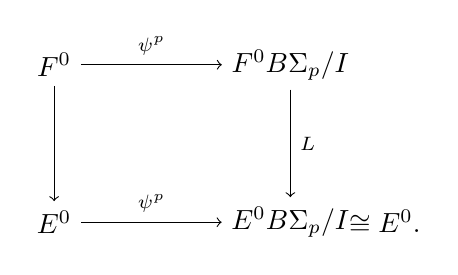
\begin{tikzpicture}
	\node (LT) at (0, 2) {$F^0$};
        \node (LB) at (0, 0) {$E^0$};
	\node (RT) at (3, 2) {$F^0 B\Sigma_p/I$};
	\node (RB) at (3, 0) {$E^0 B\Sigma_p/I$};
	\node at (4.2,0) {$\cong E^0.$}; 
	\draw [->] (LT) -- node [above] {$\scriptstyle \psi^p$} (RT); 
	\draw [->] (LB) -- node [above] {$\scriptstyle \psi^p$} (RB); 
	\draw [->] (LT) -- (LB); 
	\draw [->] (RT) -- node [right] {$\scriptstyle L$} (RB);
\end{tikzpicture}
\end{center}
Recall that the top operation arises from the universal deformation 
of Frobenius, which is represented by the ring $\CO_{X_1} = F^0 B\Sigma_p/I$, 
where $I = \sum_{0<i<p} {\rm Image}\big(E^0 B(\Sigma_i\times\Sigma_{p-i}) 
\xrightarrow{\text{transfer}} E^0 B\Sigma_{p}\big)$ is 
the transfer ideal.  The vertical maps are induced by the $K(1)$-localization 
$F \to E$.  In terms of homotopy groups, it is obtained by inverting 
the height 2 generator $v_1$ and completing at the ideal $(p)$, ie 
$F^0 = {\mb W}k \llbracket v_1,...,v_{n-1} \rrbracket$ and 
$E^0 = {\mb W}k \llbracket v_1,...,v_{n-1} \rrbracket [v_1^{-1}]_p^\wedge$.  
For example, $\pi_0 L_{K(1)} E_2 = \varprojlim {\mb Z} (\!(a)\!) /(2^i) = 
\{\sum_{n = -\infty}^{\infty} c_n a^n | c_n \in {\mb Z}_2, c_n \to 0 \text{~2-adically as~} n \to -\infty\}$.  
In particular, the formal group of $F^0$ obtains a unique degree $p$ 
subgroup after being pulled back to $E^0$, and the map $L$ classifies it.  
We will explain this uniqueness of subgroup and the isomorphism at the 
bottom right corner shortly.  

In order to do explicit calculation, we need to examine $L$ more 
carefully.  For a $p$-divisible group $\mb G$ over a base scheme $X$, 
the restriction of $\mb G$ to any geometric point $x \in X$ lives in 
the natural short exact sequence 
$0 \to \mb G^{\text{for}} \to \mb G_x \to \mb G^{\text{\'et}} \to 0$ 
with the subobject (the connected component of the identity) the
{\em formal} component and the quotient the {\em \'etale} component.  The
formal component $\mb G^{\text{for}}$ is a formal group on $X$.  The localization 
$L$ factors through $E^0 \otimes_{F^0} F^0 B\Sigma_p/I$, and along the base change 
$F^0 B\Sigma_p/I \to E^0 \otimes_{F^0} F^0 B\Sigma_p/I$ the $p$-divisible 
group consisting solely of formal component may split into formal and \'etale components.  
We want to take the formal component so that the unique 
subgroup classified by $L$ lands in the formal group over $E^0 B\Sigma_p/I$.  

\begin{exam}
\label{ex:h1p2}
We continue example \ref{ex:h2p2} in the $K(1)$-local setting.  After base 
change to $L_{K(1)} E_2$, the universal elliptic curve $C$ has a 
unique degree 2 subgroup in its formal component, 
which is the canonical subgroup introduced in \cite{lubin}.  
To be explicit, the degree 2 subgroup generated by $(d,-d^3)$ 
is contained in the formal component if and only if $(d,-d^3)$ 
is in the formal neighborhood of the identity $(0,0)$.  The 
equation $d^3 - a d - 2 = 0$ which parametrizes degree 2 subgroups has a unique root in ${\mb F}_2 (\!(a)\!)$, 
and Hensel's lemma implies that this lifts to a root in $\pi_0 L_{K(1)} E_2 \cong {\mb Z}_2 (\!(a)\!)$.  
Plugging this specific value of $d$ into 
$\psi^2\co \pi_0 E_2 \to \pi_0 E_2 [d]/(d^3-ad-2)$, we get an 
endomorphism of the ring $\pi_0 L_{K(1)} E_2$, and this 
endomorphism is the $K(1)$-local power operation.  For an 
application of this calculation, see \cite[section 6]{level3}.
\end{exam}

Lastly we note that the above commutative square describes the 
pattern for $K(m)$-local operations with $m > 1$ as well, but the 
isomorphism at the bottom right corner, namely the uniqueness of 
the degree $p$ subgroup after localization, is specific to the height 1 case.

\begin{lem}
$E^0 B\Sigma_p/I \cong E^0$.
\end{lem}
We can interpret this isomorphism as generalizing what we have 
seen in example \ref{ex:K} about the multiplicative formal group: a formal group $\mb G$ of height 1 
has a unique degree $p$ subgroup given by ${\mb G}[p]$, and 
thus the ring $E^0 B\Sigma_p/I$ classifying subgroup of degree 
$p$ is isomorphic to $E^0$ so that the power operation takes 
the form $\psi^p\co E^0 \to E^0$ which is a lift of Frobenius.  
In general a height $n$ formal group has $(p^n-1)/(p-1)$ degree 
$p$ subgroups, as can be seen from the calculations in the proof 
below, and in the example of section \ref{sec:p3} where $n=2$ 
and $p=3$.
\begin{proof}
First we identify $E^0 B\Sigma_p$ as the subset of $E^0 BC_p$ fixed by 
the action induced by ${\rm Aut} C_p \cong {\mb F}_p^\times$. This is 
a special case of the calculations in \cite[section 12]{lpo}.  
We have
\[
 B\Sigma_p \stackrel{\rm tr}{\longrightarrow} BC_p \stackrel{\rm res}{\longrightarrow} B\Sigma_p,
\]
where $\rm tr$ is the transfer map, and $\rm res$ is the restriction 
map.  Since $[\Sigma_p : C_p]$ 
is prime to $p$, the composite is a $p$-local equivalence, and thus 
$p$-locally $B\Sigma_p$ is a retract of $BC_p$.  Moreover, ${\rm Aut} C_p$ 
acts on $\Hom (C_p,\Sigma_p)$ by precomposing, which induces homotopic 
maps $BC_p \to B\Sigma_p$, and thus the same map $E^0 B\Sigma_p \to E^0 BC_p$.  
We can calculate $E^0 BC_p$ by considering the pullback square 
\begin{center}
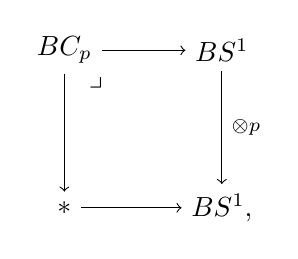
\begin{tikzpicture}
	\node (LT) at (0, 2) {$BC_p$};
        \node (LB) at (0, 0) {$*$};
	\node (RT) at (2, 2) {$BS^1$};
	\node (RB) at (2, 0) {$BS^1$,};
	\node at (0.4, 1.6) {$\lrcorner$};
	\draw [->] (LT) -- (LB);
	\draw [->] (LT) -- (RT);
        \draw [->] (LB) -- (RB);
	\draw [->] (RT) -- node [right] {$\scriptstyle \otimes p$} (RB);
\end{tikzpicture}
\end{center}
where the right-hand vertical map sends the tautological line bundle to 
its $p$th tensor power.  Applying $E^0(-)$ we have a pushout square 
where the right-hand vertical map becomes $[p]\co E^0 \llbracket u \rrbracket \to E^0 \llbracket u \rrbracket$ 
with $u$ the first Chern class of the tautological line bundle and $[p](u)$ 
the $p$-series of the formal group law of $E$.  Thus $E^0 BC_p \cong E^0 \llbracket u \rrbracket / \big([p](u)\big)$, 
where $[p](u) = p u + \cdots + v_1 u^p + \cdots$ with $v_1$ invertible in $E^0 \cong {\mb W}k \llbracket v_1,...,v_{n-1} \rrbracket [v_1^{-1}]_p^\wedge$.  
For $q \in {\mb F}_p^\times$, the induced action on $E^0 BC_p$ sends $u$ to $[q](u) = q u + \cdots$.  
Hence $E^0 B\Sigma_p \cong (E^0 BC_p)^{{\rm Aut} C_p} \cong E^0 \oplus \big(E^0 \cdot \prod_{q=1}^{p-1} [q](u)\big) = E^0 \oplus \big(E^0 \cdot (u^{p-1} + \cdots)\big)$.  

Next we identify the transfer ideal $I = \sum_{0<i<p} {\rm Image}\big(E^0 B(\Sigma_i\times\Sigma_{p-i}) 
\xrightarrow{\text{transfer}} E^0 B\Sigma_{p}\big)$ 
as the second summand in $E^0 B\Sigma_p$.  Similarly as above, for all 
$0 < i < p$, the composite
\[
 E^0 B(\Sigma_i \times \Sigma_{p-i}) \stackrel{\rm res}{\longrightarrow} E^0 \stackrel{\rm tr}{\longrightarrow} E^0 B(\Sigma_i \times \Sigma_{p-i})
\]
is the identity, and thus $E^0 B(\Sigma_i \times \Sigma_{p-i}) \cong E^0$.  
Moreover, by the ``double-coset formula'' the composite 
\[
 E^0 \stackrel{\rm tr}{\longrightarrow} E^0 B\Sigma_p \stackrel{\rm res}{\longhookrightarrow} E^0 BC_p
\]
has image the same as $E^0 \stackrel{\rm tr}{\longrightarrow} E^0 BC_p$.  Thus $I$ is generated by 
${\rm tr}(1)$ as an $E^0$-module.  Write $E^0 BC_p = E^0 \llbracket u \rrbracket / \big( [p](u) \big) = E^0 \llbracket u \rrbracket / \big( u \cdot \langle p \rangle(u) \big)$, 
where $\langle p \rangle(u) = p + \cdots + v_1 u^{p-1} + \cdots$, and 
write ${\rm tr}(1) = f(u) \in E^0 \llbracket u \rrbracket$ by abuse of notation.  Since the composite 
\[
 E^0 \stackrel{\rm tr}{\longrightarrow} E^0 BC_p \stackrel{\rm res}{\longrightarrow} E^0
\]
is multiplication by $p$, $f(0) = {\rm res}\big( f(u) \big) = {\rm res}\big( {\rm tr}(1) \big) = p$.  Moreover 
$u \cdot f(u) = u \cdot {\rm tr}(1) = {\rm tr}\big( {\rm res}(u) \big) = {\rm tr}(0) = 0$, and thus $u \cdot f(u)$ 
is divisible by $[p](u)$.  We claim that $f(u) = \langle p \rangle (u)$.  Clearly 
$\langle p \rangle(u)$ starts with $p$ and is annihilated by $u$ in $E^0 \llbracket u \rrbracket / \big( u \cdot \langle p \rangle(u) \big)$.  
Applying the snake lemma to two rows of copies of
\[
 0 \longrightarrow E^0 \llbracket u \rrbracket \stackrel{\cdot u}{\longrightarrow} E^0 \llbracket u \rrbracket \longrightarrow E^0 \longrightarrow 0,
\]
with vertical maps being multiplication by $[p](u)$ on $E^0 \llbracket u \rrbracket$ and zero on $E^0$, 
we see that every element annihilated by $u$ is a multiple of $\langle p \rangle(u)$ by an element of $E^0$.  
As $p$ is not a zero-divisor in $E^0$, the claim follows.  Thus $I = E^0 \cdot \langle p \rangle(u)$.  As $v_1$ is 
invertible in $E^0$, $E^0 B\Sigma_p / \big( \langle p \rangle(u) \big) \cong E^0$.
\end{proof}

We also note that at height 1, as in example \ref{ex:K}, the power 
operation $\psi^p$ determines the other operations $\psi^{p^r}$ for 
$r > 1$ by self composition.  Thus in the $K(1)$-local setting it 
suffices to study only $\psi^p$ as above, and for this reason we 
will simply write $\psi$ for {\em the} $K(1)$-local power operation.  
At higher height, the relationship among these operations is more 
complicated.  


\section{Power operations at the prime 3}
\label{sec:p3}


In \cite{h2p2}, Rezk gives explicit calculations of the algebraic 
theory of power operations for a specific Morava $E$-theory of height 
2 at the prime 2 (cf example \ref{ex:h2p2}).  We record some 
calculations mimicking some of the results there, at the prime 3, 
together with calculations of the corresponding $K(1)$-local power 
operation.  Many ideas in carrying out 
these calculations were suggested by the author's advisor, Tyler Lawson.  

The Morava $E$-theory $F$ of height 2 we consider here is associated to the 
deformations of a supersingular elliptic curve over ${\mb F}_3$.  Our 
calculations break into the following steps:
\begin{enumerate}
\item Find the universal elliptic curve with a choice of 4-torsion 
point, so that a posteriori the supersingular elliptic curve that we are interested in 
is the one with the Hasse invariant zero; 
\item Study the degree 3 subgroups of this elliptic curve - in 
particular, we need to compute 
\begin{itemize}
 \item the coordinate ring parametrizing degree 3 subgroups,  
 \item the equation of the quotient curve as 
the image of the universal degree 3 isogeny;
\end{itemize} 
\item $K(1)$-localize.  
\end{enumerate}
We try to make the calculations along a general recipe in hope of adaptibility to larger primes.


\subsection{The universal elliptic curve with a choice of 4-torsion point}
\label{subsec:step1}

First we note that a supersingular elliptic curve over ${\mb F}_3$ 
cannot have a 3-torsion point, and in order to have a unique lift of 
the elliptic curve together with a choice of $N$-torsion point along 
a deformation of $k = {\mb F}_3$ to a complete local ring $R$ with 
residue field containing $k$, $N$ must be prime to 3.  As the 
associated moduli stack ${\cal M}\big(\Gamma_1(2)\big)$ to a level
$\Gamma_1(2)$-structure on the elliptic curve is not representable 
by a scheme due to the existence of nontrivial 
automorphism of order 2, the natural choice for the universal elliptic 
curve is one equipped with a level $\Gamma_1(4)$-structure.  

The computation for the equation of the universal elliptic curve with 
a choice of 4-torsion point $P$ is analogous to 
\cite[proposition 3.2]{tmf3}, where the universal elliptic curve used for the prime 2 
case has a choice of 3-torsion point.  In the $xy$-coordinates, 
with the constraints that $P$ be at the origin, $2P$ be on the 
$x$-axis, and $4P$ be the identity $O$, we have the affine Weierstrass 
equation 
\[
 y^2 + a x y + a c y = x^3 + c x^2
\]
over the graded ring ${\mb Z}_{(3)}[a,c]$, where $|a| = 1$ and $|c| = 2$.  
The grading comes from the action of $\Gm = \Spec {\mb Z}[\lambda^{\pm1}]$ 
given by $a \mapsto \lambda a$ and $c \mapsto \lambda^2 c$.  By 
\cite[theorem 4.1(a)]{AEC}, the Hasse invariant can be computed as 
$h = a^2 + 4c$, so that the curve is supersingular precisely when $h = 0$.  To facilitate 
calculation, we work in the affine coordinate chart $c = 1$ of 
${\cal M}\big(\Gamma_1(4)\big)$ so that the elliptic curve is given by 
\[
 y^2 + a x y + a y = x^3 + x^2,
\]
with $\Delta = a^2(a + 4)(a - 4)$ and $h = a^2 + 4$.  This reduction is analogous to the one 
discussed in detail in \cite[section 4]{level3}.  In $uv$-coodinates, with 
$u = x/y$ and $v = 1/y$, this is 
\[
 v + a u v + a v^2 = u^3 + u^2 v,
\]
which is the form we will use most often later.  We denote this elliptic curve by $\cal E$.  

We note that $\cal E$, together with the universal elliptic curve with a choice of 3-torsion point studied in \cite{tmf3} and \cite{h2p2}, give models 
for {\em all} primes.  


\subsection{Degree 3 subgroups}
\label{subsec:step2}

Given the elliptic curve 
\[
 {\cal E}\co y^2 + a x y + a y = x^3 + x^2,
\]
$(x,y)$ is a 3-torsion point 
if and only if the division polynomial 
\[
 \psi_3 (x) = 3x^4 + (a^2 + 4) x^3 + 3a^2 x^2 + 3a^2 x + a^2 = 0
\]
(cf \cite[exercise 3.7(d)]{AEC}; this polynomial is exactly what one gets for the 
characterization, away from the prime 2, of a flex point in terms of the second 
derivative $y''$ calculated by implicit differentiation).  We want to translate this into the $uv$-coordinates, 
which are more convenient to work with explicitly in the formal neighborhood of the identity 
(in $xy$-coordinates, the identity is at $\infty$), and get a ``characteristic'' equation 
comparable to $d^3 - a d - 2 = 0$ in example \ref{ex:h2p2}, where $d$ was the $u$-coordinate of a 2-torsion point.  
From the formula of multiplication-by-3 in the $xy$-coordinates, we have
\[
 [3](u,v) = \big(\frac{\phi_3(\frac{u}{v})\psi_3(\frac{u}{v})}{\omega_3(\frac{u}{v})},\frac{\psi_3(\frac{u}{v})^3}{\omega_3(\frac{u}{v})}\big),
\]
with notation following \cite[exercise 3.7(d)]{AEC}, and thus our preliminary equation is $\psi_3(\frac{u}{v}) = 0$.  
Clearing the denominators in $\psi_3(\frac{u}{v})$ , we get 
\[
 \psi_3'(u,v) = 3u^4 + (a^2 + 4) u^3 v + 3a^2 u^2 v^2 + 3a^2 u v^3 + a^2 v^4.
\]
To eliminate $v$, we multiply the ``conjugate'' $\psi_3'(u,v')$, where $v$ and $v'$ are conjugate roots of the quadratic equation 
\[
 a v^2 + (1 + a u - u^2) v - u^3 = 0
\]
coming from the equation of $\cal E$.  
We get a degree 8 polynomial in $u$:
\[
 f(u) = -3 - 3 a u + 8 u^2 - a^2 u^2 + 9 a u^3 - 6 u^4 + 6 a^2 u^4 + 7 a u^5 +
  a^3 u^5 + 3 a^2 u^6 + 3 a u^7 + u^8.
\]
Thus a 3-torsion point $(d,e)$ must satisfy $f(d) = 0$.  

We note that according to section \ref{sec:K(1)}, in particular example \ref{ex:h1p2}, 
$f(u)$ should have a unique root reduced to zero modulo 3 after $h = a^2 + 4$ gets inverted.  
We compute that 
\[
 f(u) \equiv u^2 (u + a)^6~~\text{mod}~3,
\]
and in view of $a \not\equiv 0$ by the nonsingularity 
of $\cal E$ (recall that $\Delta = a^2(a + 4)(a - 4)$), such a root has multiplicity 2.  
Thus $f(u)$, extracted out of a conjugation procedure, is not ideal in this aspect.  This is the best 
possible polynomial solely about $u$ we have at this point, and in later steps we will have to improve and ``rescale'' it back to a degree 4 polynomial.  

Next we want to express $e$ in terms of $d$.  At the prime 2 (cf example \ref{ex:h2p2}), 
the relation $e = -d^3$ can be obtained, for example, by manipulating the division polynomial 
$\psi_2$ and its ``conjugate'' as above, or simply by computing the inversion formula 
for a 2-torsion point on the elliptic curve as in \cite{h2p2}.  The prime 3 
case is a little more involved.  Using the Euclidean algorithm, we compute the gcd of 
\[
 A(v) = \psi_3'(u,v) = 3u^4 + (a^2 + 4) u^3 v + 3a^2 u^2 v^2 + 3a^2 u v^3 + a^2 v^4
\]
and 
\[
 B(v) = a v^2 + (1 + a u - u^2) v - u^3~~~~\text{(equation of $\cal E$)},
\]
both of which vanish at $(d,e)$.  We have
\[
 A(v) = B(v)Q_1(v) + R_1(v)
\]
\[
 ~~~B(v) = R_1(v)Q_2(v) + R_2(v),
\]
and it turns out that $R_2(e) = 0$ as a result of $f(d) = 0$.  Thus
\[
 R_1(d,e) = p(d) + q(d) e = 0
\]
is a relation between $d$ and $e$, linear in $e$.  We have explicit formulas for $p(d)$ and $q(d)$, 
and we can compute the inverse of $q(d)$ by applying the Euclidean algorithm to find 
\[
 1 = a(d)q(d) + b(d)f(d) = a(d)q(d).
\]
In the end we have a degree 14 polynomial $e = g(d)$, comparable to $e = -d^3$ in the prime 2 case.  

Now we are ready to compute the universal degree 3 isogeny and thus the equation of the quotient curve, 
from which we can find an explicit formula for the power operation $\psi^3\co F^0  \to F^0 [d] / \big(f(d)\big)$, where $F^0 = {\mb Z}_3 \llbracket h \rrbracket$
(to be precise, the target should actually be a certain improved coordinate ring as promised earlier).  

We follow the ``Lubin isogeny'' construction (cf \cite[proof of theorem 1.4]{lubin}) to compute the coordinates $(u',v')$ of the isogeny as follows.  
Let $P\big(u,v(u)\big)$ be a general point on $\cal E$, and $Q\big(d,e(d)\big)$ be a 3-torsion point.  For 
$v(u)$, we use an appoximation with the first few terms (up to at least degree 9 for our purpose) 
from the power series expansion of one of the roots (the one lying in the formal neighborhood of the identity, ie $v(0)=0$) of the quadratic equation 
\[
 a v^2 + (1 + a u - u^2) v - u^3 = 0;
\]
for $e(d)$, we use the polynomial $g(d)$ computed above.  We set 
\[
 u' = u(P) u(P-Q) u(P+Q),
\]
and similarly for $v'$.  By computing the inversion and addition formulas for the curve $\cal E$, 
we can write down explicit formulas for $u' = \alpha u + \cdots$ and $v' = \beta u^3 + \cdots$ in terms of the 
uniformizer $u$ and parameters $a$ and $d$.  We note that in order to have the equation of the quotient curve in Weierstrass form, 
we need to include an adjusting constant factor $\alpha^3 / \beta$ into $v'$, comparable to the term $-1$ appearing in the formula for $u'$ in \cite{h2p2}.  
We then solve for the Weierstrass equation which $u'$ and $v'$ satisfy so that the equation of the quotient curve turns out to be 
\[
 v + r u v + r v^2 = u^3 + u^2 v,
\]
where

$r(a,d) = -\frac{1}{(-4 + a) (4 + a)}(-126 a + 28 a^3 - a^5 + 120 d - 9 a^2 d + 3 a^4 d + 258 a d^2 -
  67 a^3 d^2 + 3 a^5 d^2 - 152 d^3 + 208 a^2 d^3 - 40 a^4 d^3 +
  a^6 d^3 + 198 a d^4 - 33 a^3 d^4 - 3 a^5 d^4 + 8 d^5 + 63 a^2 d^5 -
  15 a^4 d^5 + 70 a d^6 - 17 a^3 d^6 + 24 d^7 -
  6 a^2 d^7)$

(note that $(-4 + a) (4 + a)$ is invertible as $\Delta = a^2(a + 4)(a - 4)$).  Hence 
$\psi^3(a) = r(a,d)$ gives the power operation, and we check that 
it reduces to $a^3$ modulo 3 (the Frobenius congruence at height 1 over ${\mb F}_3$), as $d \equiv 0$ mod 3.  

Lastly we compute the coordinate ring as the target of the power operation $\psi^3$.  
Set $t = g(d)/d$, which is the inverse of the $x$-coordinate of a 3-torsion point.  
This is a quantity which is invariant under negation using the group law 
of $\cal E$ (as we have $[-1](x) = x$) and is ``distinguishable'' from the identity in its formal neighborhood (in the $xy$-coodinates the identity is at $\infty$).  
Given that $f(d) = 0$, we compute that $t$ is the root of a quartic polynomial 
\[
 w(t) = a^2 t^4 + 3 a^2 t^3 + 3 a^2 t^2 + (a^2 + 4) t + 3,
\]
which has a unique root reduced to zero modulo 3.  We note that via the 
relation $t = 1/x$ this polynomial recovers the division polynomial 
$\psi_3(x)$.  Thus the eight roots of $f(d)$ together with $d = 0$ 
correspond to the nine 3-torsion points on $\cal E$, and the four roots 
of $w(t)$ correspond to the four degree 3 subgroups consisting of 
3-torsion points, one of which lies in the formal neighborhood of the 
identity.  In particular, the equation of $\cal E$ implies that $d$ 
satisfies a quadratic equation in terms of $t$: 
\[
 (t + 1) d^2 - a t (t + 1) d - t = 0.
\]
From this equation and $w(t) = 0$, we can rewrite 
$\psi^3(a) = r(a,d)$ above in terms of $t$. 
\begin{prop}
 The universal degree 3 isogeny with source $\cal E$ is defined over the ring
$F^0[\Delta^{-1}][t]/\big(a^2 t^4 + 3 a^2 t^3 + 3 a^2 t^2 + (a^2 + 4) t + 3\big)$, 
and has target the elliptic curve 
\[
 y^2 + r x y + r y = x^3 + x^2,
\]
where $r(a,t) = a^3 t^3 + 3 a^3 t^2 + 3 a^3 t - 4 a t + a^3 - 3 a$.  
The kernel of this isogeny is generated by the 3-torsion point with $x$-coordinate $1/t$.  
Thus the power operation $\psi^3$ is given by 

$\psi^3(a) = (t + 1)^3 a^3 - (4 t + 3) a$,

$\psi^3(h) = (t + 1)^3 h^3 - (22 t^3 + 69 t^2 + 75 t + 27) h^2 + (128 t^3 + 424 t^2 + 512 t + 201) h - 16 (14 t^3 + 49 t^2 + 65 t + 27)$.
\end{prop}


\subsection{$K(1)$-localize}
\label{subsec:step3}

As in example \ref{ex:h1p2}, with $h = a^2 + 4$ invertible, we can 
solve for $t$ 3-adically from the equation $w(t) = 0$ by first writing 
\[
 t = -\frac{1}{a^2 + 4}(a^2 t^4 + 3 a^2 t^3 + 3 a^2 t^2 + 3),
\]
and then substituting $t$ recursively.  Plugging this uniquely determined 
value of $t$ into $\psi^3(h,t)$ computed above, 
we get the $K(1)$-local power operation $\psi$ as an endomorphism of the 
ring $E^0 = {\mb Z}_3 (\!(h)\!) [\Delta^{-1}]_3^\wedge$.  


\nocite{*}
\bibliography{po}
\end{document}
